% !Mode:: "TeX:UTF-8"

%%% 此部分包含: (1) 英文封面 (无需改动) ; (2) 郑重声明 (无需改动).

%%%%%%%%%%%%%%%%%%%%%%%%%%%%%
%%% -------------  英文封面 (无需改动)-------------   %%%
%%%%%%%%%%%%%%%%%%%%%%%%%%%%%
\thispagestyle{empty}
\renewcommand{\baselinestretch}{1.5}  %下文的行距
\vspace*{0.5cm}

\begin{center}{\zihao{2} \the\Etitle \par}\end{center}

\vfill

\begin{center}
\zihao{4}
\begin{tabular}{ r l }
 Candidate:      &  {\sc \the\Eauthor} \\
 Student Number: & {\the\StudentNumber} \\
 Supervisor:     &  {\sc \the\Esupervisor}
\end{tabular}

\vspace*{2cm}
\begin{center}
  \iflib % 向图书馆提交电子文档, 使用黑白校徽.
  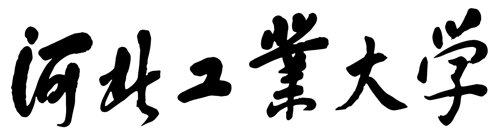
\includegraphics[height=4cm]{hebut.png}       %%  黑白的. 很小, 只有 10k.
  \else
     \ifprint % 文档打印, 使用黑白校徽.
  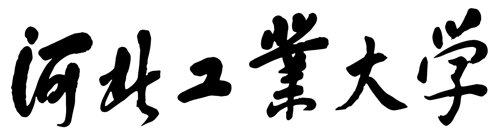
\includegraphics[height=4cm]{hebut.png}       %%  黑白的.
  \else
  
\includegraphics[height=4cm]{hebut1.png} %%  彩色的.
  \fi
  \fi
\end{center}


\zihao{-2}
\the\Schoolname\\
{\sc Hebei University of Technology}

\vspace*{1.0cm}

\the\Edate

\end{center}
%%%%%%%--判断是否需要空白页-----------------------------
 \iflib
 \else
\newpage
\thispagestyle{empty}
 \cleardoublepage
 \fi
%%%%%%%-------------------------------------------------
%%%--- 加入``郑重声明'' --- %%%%%%%%%%%%%%%%%
{\pagestyle{empty}
\newpage
\vspace*{20pt}
\begin{center}{\ziju{0.8}\zihao{-2}\heiti 论文原创性声明}\end{center}
\par\vspace*{30pt}
\renewcommand{\baselinestretch}{2}
{\zihao{4} \songti %


本人郑重声明: 所呈交的论文, 是本人独立进行研究工作所取得的研究成果.
除文中已经标明引用的内容外, 本论文不包含任何其他个人或集体已经发表或撰写过的研究成果.
对本文的研究做出贡献的个人和集体, 均已在文中以明确方式标明. 本声明的法律结果由本人承担.


\vskip2cm

\hspace*{4cm}学位论文作者(签名): \hspace{4cm} \hfill \\[1cm]
\hspace*{10cm}年 \hfill  月 \hfill 日\hspace{1cm}\hfill\par}

%%%%%%%--判断是否需要空白页-----------------------------
  \iflib
  \else
  \newpage
  \cleardoublepage
  \fi
%%%%%%%-------------------------------------------------
}
\renewcommand{\baselinestretch}{1.6}
\small\normalsize




